%\chapter{流量统计设施的部署}
在前几章,我们使用CountMax解决了数据平面上流量统计的获取问题,接下来我们从控制平面探讨流量统计该如何部署。

第\ref{sec:coop}节提出了一个协作式的简单的部署策略,将计算负载均摊给所有入口和出口交换机。
但是在现实网络中的情况更加复杂,简单的协作式很可能不能满足需求,因此我们寻求在控制平面进行更优化的部署。
\chapter{GMSC:流量测量的分布式部署算法}\label{chap:gmsc}
在第\ref{chap:countmax}章,我们使用CountMax解决了数据平面上流量统计的获取问题,并提出了一个无需控制平面干预的简易部署方式——协作式CountMax。

接下来我们从控制平面出发,更进一步地探讨流量测量的分布式部署。
本章首先对问题进行形式化建模和描述,随后提出了一种名为GMSC的解决算法,最后利用仿真模拟对其进行了测试。

\chapter{最大化流统计覆盖问题}
\chapter{GMSC:流统计覆盖的解决算法}\label{chap:gmsc}
在本章,我们提出一个简单但有效的算法解决MSC问题,称为GMSC。

\section{算法设计}\label{sec:gmsc}
如第\ref{sec:mscdef}节中定理\ref{thm:nphard}的证明,在只考虑交换机$v_i$的情况下,MSC问题退化为单背包问题。
我们可以对每个交换机分别求解单背包问题,获得每个交换机的最大容纳价值,记为$p(v_i)$。
接下来选择$p(v_i)$最大的那个交换机,将背包问题的解应用到此交换机上。
最后,由于这个交换机被分配了掩码,要相应的更新这些掩码在其余交换机上的价值。
重复这个过程,直到所有交换机都被分配过为止。

这是一个贪心(Greedy)算法,因而称其为GMSC。
\begin{algorithm}[htb]
    \small
    \SetAlgoLined
    \KwData{$V$:交换机的集合;$F$:覆盖的所有流的集合}
    $F=\Phi$\;
    \While{$|V|>0$}{
        \ForEach{$V$中的交换机$v$}{
            求解单背包问题,得到$v$的最大价值$p(v)$和对应的解$S(v)$。记$S(v)$中覆盖的流的集合为$F(v)$\;
        }
        找出$m$,使$p(v_m)$最大\;
        将$S(v_m)$中的掩码应用到$v_m$上\;
        将$F(v)$中覆盖的流加入$F$\;
        从$V$中移除$V_m$\;

        \ForEach{$V$中的交换机$v_i$}{
            \ForEach{$\Omega$中的掩码$r_j$}{
                更新$p(\Pi_i^j)$,去除$\Pi_i^j \cap F(v)$部分的价值\;
            }
        }
    }
    \caption{GMSC}
    \label{alg:count_max}
\end{algorithm}

\section{单背包问题的解法}
作为一个经典问题,单背包问题有多种不同的解法,其中最经典的是动态规划法 \cite{martello1999dynamic}和贪心法\cite{cmulec10}。
这两种解法在各类算法教科书中都能轻易找到,因此不再赘述。
设背包容量为$B$,可选择的物品数为$m$,则动态规划法的时间复杂度是$O(m\cdot B)$,近似比为1;
贪心法的时间复杂度是$O(m \log{m})$,近似比为1/2。

\section{GMSC的性能分析}
\subsection{近似性能}
\begin{theorem}\label{tm:gmscappr}
    GMSC的近似比为$\frac{\mu}{1+\mu}$,其中$\mu$为单背包问题解法的近似比。
\end{theorem}

\begin{proof}
令$Q_G$表示通过GMSC所覆盖的流,$G_l$表示GMSC在第$l$次迭代后所覆盖的流,则$Q_G = G_n$。
令$X_l$代表第$l$次迭代中所选择的掩码带来的价值增量,则$X_l =w(G_l \backslash \bigcup\nolimits^{l-1}_{i=1}G_i)$。

考虑GMSC已经完成$l-1$轮迭代的情况。在第$l$轮中,GMSC选择了交换机$v^l$和其上的流$X_l$。
作为对比,最优解法也一定会从$v^l$中选择一个掩码的集合,其中包含的流的集合记为$O_l$。
设最优解法最终覆盖的流的集合为$OPT$,则$OPT = \bigcup\nolimits_{l=1}^{n}O_l$。
如果在这一轮,我们选择$O_l$而不是$X_l$的话,则这一轮的价值增量为$w(O_l \backslash \bigcup\nolimits^{l-1}_{i=1}G_i)$,记为${X'}_l$。

设在已完成$l-1$轮的情况下,$v^l$上的背包问题的最优解是$Y_l$,则根据近似比的定义有$X_l \ge \mu Y_l$。
又因为$Y_l$是当前情况下的短视最优解,故$Y_l \ge {X'}_l$。
因而我们有:

\begin{align}
    X_l &\ge \mu Y_l \notag\\
        &\ge \mu {X'}_l \notag\\
        &= \mu \cdot w(O_l \backslash \bigcup\nolimits^{l-1}_{i=1}G_i) \notag\\
        &\ge \mu \cdot w(O_l \backslash Q_G) \notag
\end{align}

根据$Q_D$和$OPT$的定义,有:
\begin{align}
    w(Q_D)&=\sum\nolimits_{l=1}^{n} X_l \notag\\
        &\ge \sum\nolimits_{l=1}^{n} \mu \cdot w(O_l \backslash Q_D) \notag\\
        &=  \mu \cdot \sum\nolimits_{l=1}^{n} w(O_l \backslash Q_D) \notag\\
        &\ge \mu \cdot w ((\bigcup\nolimits_{l=1}^{n}O_l) \backslash Q_D) \notag\\
        &=  \mu \cdot w( OPT \backslash Q_D) \notag\\
        &\ge \mu \cdot [ w(OPT)-w(Q_D)] \notag
\end{align}

因而:
\begin{equation}\label{eq:gmscappr}
    w(Q_D) \ge \frac{\mu }{1+\mu} \cdot w(OPT)
\end{equation}
定理\ref{tm:gmscappr}得证。
\end{proof}

\section{时间复杂度}
若单背包问题的解法的时间复杂度为$O(\rho)$,更新一个掩码的价值的时间复杂度为$O(\tau)$,则GMSC的时间复杂度为$O(n^2\cdot m \cdot \tau + n^2 \cdot \rho)$。

假设一个掩码中最多有$h$个流,那么$\tau = h\cdot m$。因而:

\begin{theorem}\label{tm:gmsctime}
    GMSC的时间复杂度为$O(n^2\cdot m^2 \cdot h+ n^2 \cdot \rho)$。
\end{theorem}
\section{GMSC的仿真模拟测试}
本节使用仿真平台对GMSC的性能进行测试。具体而言,是测试GMSC能在多大程度上提升sketch测量的性能。

\subsection{测试设置}
本节中用到的测试指标为平均估计误差和最大交换机负载,
其中平均估计误差的定义与第\ref{subsec:metric}节相同。
最大交换机负载是统计每个交换机所处理的流量总和,取其最大值作为指标。
测试基准有两种,第一种是协作式CountMax,另一种是非协作式CountMax。
其中非协作式CountMax是在所有接入层交换机上都部署CountMax,每个CountMax只处理以本交换机作为出口交换机的数据包。
对于一条流被多次测量的情况,采取多个测量值的最大值作为结果。

测试拓扑采用的是与第\ref{sec:simulation}节相同的Fat-tree。
测试当中,用于计算的先验知识为所有流的准确信息和大小,掩码根据源地址与目的地址(O-D对)进行分割。
测试用的流的集合也与第\ref{sec:simulation}节相同,其中最大的一条流的大小约为9GB。
在GMSC中,每条流的价值和代价均为流的流量大小,每个交换机设置的负载上限约为10GB。

\subsection{测试结果}

\begin{figure}[ht]
	\centering
	\begin{minipage}[t]{0.48\linewidth}		
		%\begin{figure}[!t]
		\centering
		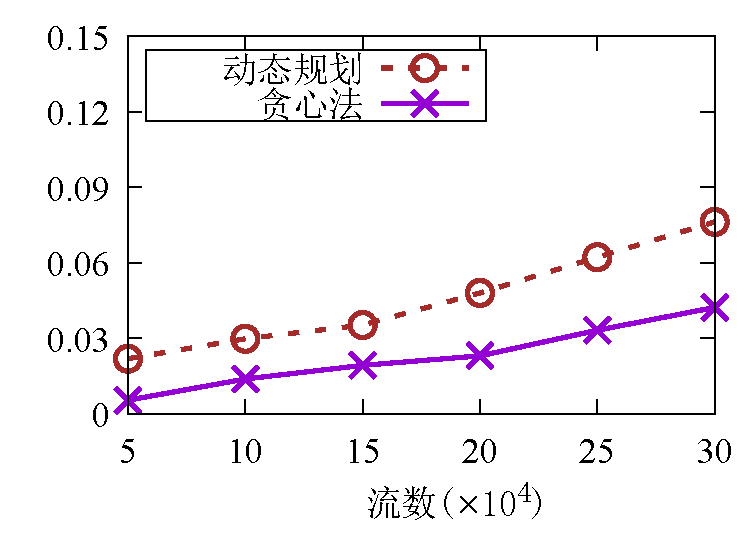
\includegraphics[width=\linewidth]{fig/msc_cmp_appr.pdf}
		\caption{\textnormal{平均估计误差与流数,$k=1000$。}}
		\label{fig:msc,appr}
		%\end{figure}
	\end{minipage}\vspace{-0.6em}\hspace{0.4em}
	\begin{minipage}[t]{0.48\linewidth}
		\centering
		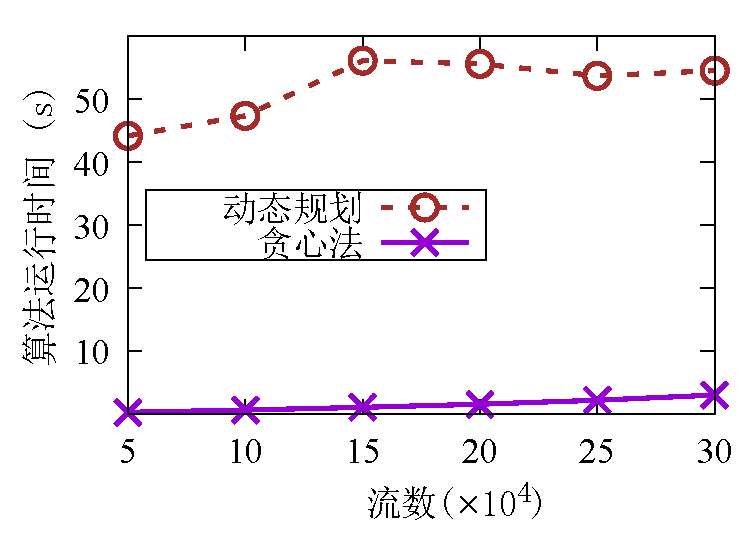
\includegraphics[width=\linewidth]{fig/msc_cmp_time.pdf}
		\caption{\textnormal{算法运行时间与流数,$k=1000$。}}
		\label{fig:msc,time}
	\end{minipage}\vspace{-0.6em}
\end{figure}

第一组测试是对比使用动态规划解背包问题的GMSC和使用贪心法解背包问题的GMSC的性能。
由于动态规划算法的时间复杂度和背包容量,即交换机负载上限呈线性关系,而测试中这一数字十分巨大,导致动态规划算法耗时极其漫长。
为了能够在合理的时间内获得结果,在这组测试中我们将流的价值和负载上限进行等比缩放(全部除以1000)后再进行动态规划。
图\ref{fig:msc,appr}中显示,由于缩放带来的误差,使用动态规划方法最终得到的估计误差反而超过了使用贪心法的误差。
图\ref{fig:msc,time}则表明,即使进行了1000倍的缩放,动态规划方法的运行时间仍是贪心法的10倍以上。
贪心法的运行时间随流数增加而增加的原因是,流数越多,每轮迭代后更新$p(\Pi_i^j)$所需的时间也会线性增加。

根据这一组实验的结果,我们决定接下来的测试中,GMSC一律使用贪心法解背包问题。

\begin{figure}[ht]
	\centering
	\begin{minipage}[t]{0.48\linewidth}		
		%\begin{figure}[!t]
		\centering
		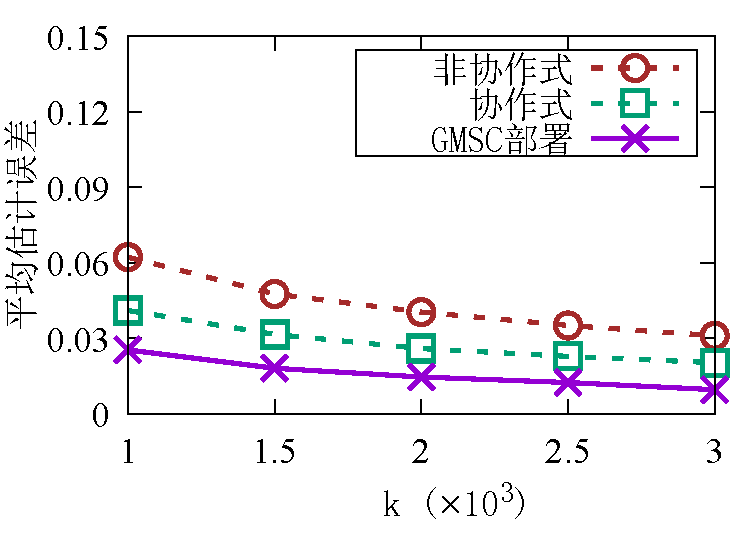
\includegraphics[width=\linewidth]{fig/msc_k_appr.pdf}
		\caption{\textnormal{平均估计误差与$k$,200000条流,$\alpha = 1\%$。}}
		\label{fig:msc,err,k}
		%\end{figure}
	\end{minipage}\vspace{-0.6em}\hspace{0.4em}
	\begin{minipage}[t]{0.48\linewidth}
		\centering
		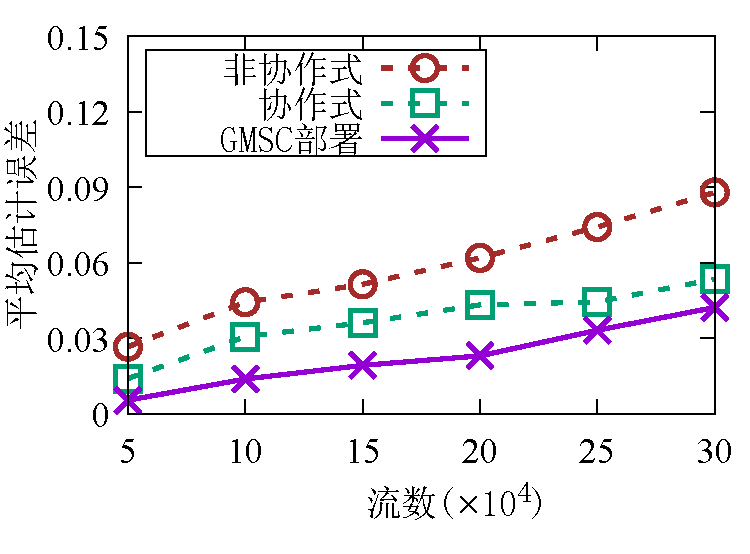
\includegraphics[width=\linewidth]{fig/msc_f_appr.pdf}
		\caption{\textnormal{平均估计误差与流数,$k=1000$,$\alpha = 1\%$。}}
		\label{fig:msc,err,flow}
	\end{minipage}\vspace{-0.6em}
\end{figure}

图\ref{fig:msc,err,k}和图\ref{fig:msc,err,flow}描述了使用GMSC部署的CountMax的估计误差与协作式和非协作式CountMax的对比。
在GMSC部署下,CountMax对网络中的大流的估计误差略有下降。和协作式CountMax相比约降低了20\%到30\%。
这主要是得益于GMSC部署将流的测量分散到各个交换机中,从而进一步减少了哈希冲突出现的概率。

\begin{figure}[ht]
	\centering
	\begin{minipage}[t]{0.48\linewidth}		
		%\begin{figure}[!t]
		\centering
		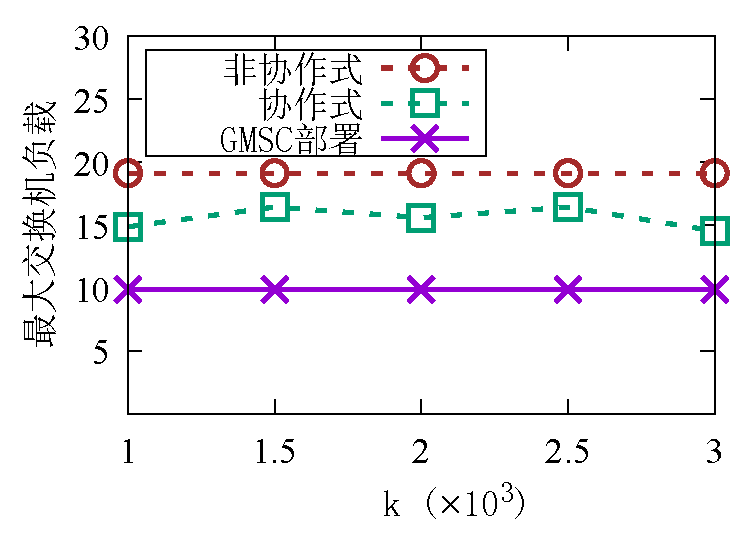
\includegraphics[width=\linewidth]{fig/msc_k_time.pdf}
		\caption{\textnormal{最大交换机负载与$k$,200000条流。}}
		\label{fig:msc,time,k}
		%\end{figure}
	\end{minipage}\vspace{-0.6em}\hspace{0.4em}
	\begin{minipage}[t]{0.48\linewidth}
		\centering
		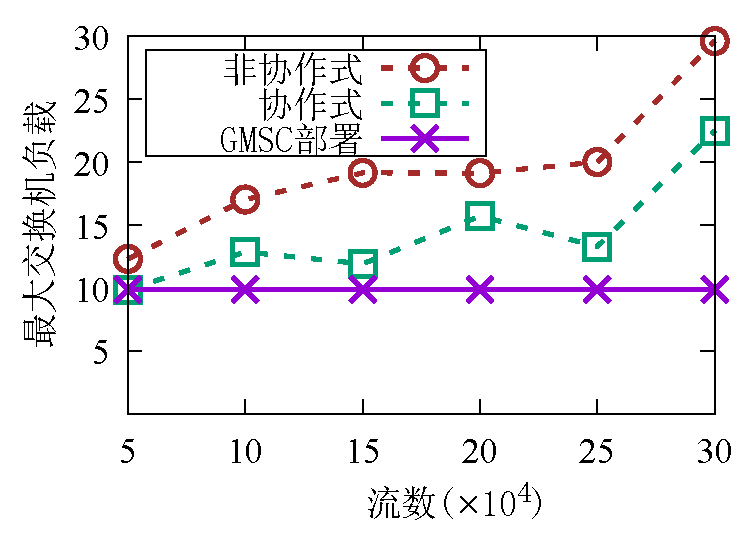
\includegraphics[width=\linewidth]{fig/msc_f_time.pdf}
		\caption{\textnormal{最大交换机负载与流数,$k=1000$。}}
		\label{fig:msc,time,flow}
	\end{minipage}\vspace{-0.6em}
\end{figure}

图\ref{fig:msc,err,k}和图\ref{fig:msc,err,flow}描述了交换机的最大负载。
由于交换机负载上限的限制,GMSC方法的最大交换机负载始终保持不变;
而协作式和非协作式的计算负载随着流数的增加明显上升,并且协作式CountMax由于引入了随机因素,导致最大交换机负载变得更加不易预测,体现在图中为较大的波动。



\section{小结}

本章首先建模分析了流量测量的分布式部署,从而提出了MSC问题并形式化定义。随后提出了GMSC算法并对其进行了分析。
最后通过仿真测试证明了GMSC的部署对CountMax的帮助。